\chapter{Introducció a l'aplicació web}

    \paragraph{}
    En aquesta secció de la memòria s’introduiran tots aquells aspectes generals referents a l’aplicació web. En concret, es tractaran els següents punts:

    \begin{itemize}
        \item Accés i codi de l’aplicació web.
        \item Requisits funcionals i no funcionals de l’aplicació web.
        \item Estructura de l’aplicació web.
        \item Estructura de l’aplicació web.
        \item Funcionament general de l’aplicació web.
        \item Detalls específics de la implementació.
        \item Certificació de l’aplicació.
        \item Google Analytics.
        \item Optimització d’imatges.
        \item Hosting de l’aplicació web.
    \end{itemize}

    \section{Accés a l'aplicació web i codi de l'aplicació}

    \paragraph{}
    L’aplicació web es troba desplegada al núvol sota l'URL:

    \begin{displayquote}
        https://pfc-family-search.herokuapp.com/
    \end{displayquote}

    Per accedir a la zona específica d’exemples, la que s’encarrega de mostrar els diferents exemples d’interacció amb l’API, fa falta utilitzar el següent usuari i contrasenya:

    \begin{itemize}
        \item \textbf{Usuari:} tum000145207
        \item \textbf{Contrasenya:} 1234pass
    \end{itemize}

    Per altra banda, el codi de les aplicacions web sol ser extens en nombre de línies i mostrar-lo en aquesta memòria resulta impossible. El codi realitzat ocupa un total de [nombre de línies] repartides un [x\%] en HTML, un [y\%] en Javascript i jQuery i un [z\%] en css.

    Tot el codi de l’aplicació pot ser trobat en el repositori GitHub accessible a través del següent URL:

    \begin{displayquote}
        https://github.com/sinh15/pfc-family-search
    \end{displayquote}

    L’estructura del codi serà presentada més endavant, en aquesta mateixa secció de la memòria, però principalment, el servidor està compost pel fitxer \emph{app.js}, els fitxers HTML es troben a la carpeta \emph{views} i els fitxers Javascript i jQuery, a la carpeta \emph{assets}.

    \section{Requisits de l'aplicació web}

    \paragraph{}
    Aquesta llista pretén oferir un tast dels requisits o manaments que s'han tingut en compte durant el desenvolupament de l'aplicació web.

    \subsection{Requisits funcionals}

    \begin{itemize}
        \item La web ha de permetre identificar-se amb FamilySearch mitjançant el sistema d'autentificació per pop-up.
        \item La web ha de permetre a l'usuari tancar la connexió amb FamilySearch mitjançant una funcionalitat de `Sign Out'.
        \item L'aplicació ha de ser capaç de tancar automàticament la connexió amb FamilySearch si aquesta expira.
        \item La web ha d'incloure una secció que ofereixi un petit resum del rerefons que va originar el projecte.
        \item La web ha de disposar d'una secció en què s'enumerin i exposin les diferents propostes de projecte generades pels futurs estudiants.
        \item L'aplicació ha d'oferir la possibilitat de cercar persones en l'arbre familiar de FamilySearch i observar-ne els detalls d'alguna en concret.
        \item L'aplicació ha de permetre a l'usuari observar l'evolució geogràfica d'un cognom donat un conjunt de països i període de temps.
        \item L'aplicació ha de permetre la visualització del nombre de naixements, casaments i defuncions enregistrades per un país al voltant d'un any concret.
        \item La secció d'exemples ha de ser només accessible si l'usuari es troba identificat a FamilySearch i ha rebut el token d'ús pertinent.
        \item En cas que el token expiri, l'usuari ha de ser redirigit a la pàgina principal en el moment d'expiració o en la seva següent interacció si aquest es troba dins de l'àrea d'exemples.
        \item L'aplicació ha d'emmagatzemar el token proporcionat per FamilySearch que rep l'usuari en un recurs que no sigui accessible ni modificable per tercers.
        \item No es permetrà a l'usuari llençar dues crides contra l’API de FamilySearch simultànies per la mateixa funcionalitat des de la mateixa pestanya del navegador.
        \item L’aplicació ha d'aportar la informació bàsica sobre l’origen del projecte i el seu rerefons. L'aplicació també ha d’enllaçar en algun lloc amb el codi font del projecte.
    \end{itemize}


    \subsection{Requisits no funcionals}

    \begin{itemize}
        \item L'aplicació web ha de funcionar i ser visualitzada de forma correcta en els principals navegadors web moderns.
        \item Els formularis de l'aplicació web que puguin generar errors han de proporcionar informació bàsica a l'usuari en el moment que el camp és abandonat o informació més detallada si envia el formulari amb errors.
        \item Els formularis de l’aplicació han de donar un feedback positiu en cas que els camps siguin omplerts de forma correcta.
        \item La web ha de ser relativament fàcil d'utilitzar, oferint les eines necessàries als usuaris i facilitant la navegació per les diferents seccions.
        \item Mentre l'aplicació web espera resposta de l’API de FamilySearch, s'ha de mostrar a l'usuari que l'aplicació es troba esperant resultats i el progrés realitzat fins al moment.
        \item L'aplicació ha de donar un feedback clar a l'usuari quan la interacció amb l’API de FamilySearch finalitza.
        \item L'aplicació ha de ser navegable de forma acceptable mitjançant dispositius mòbil. Les integracions amb l’API de FamilySearch també han de ser utilitzables, però no cal que la informació resultant es trobi completament adaptada a aquests dispositius.
        \item Les imatges de l'aplicació s'han de trobar optimitzades en la mesura que sigui possible per intentar que aquesta carregui el més ràpid possible en un entorn d'hostalatge gratuït.
        \item Les imatges principals de l'aplicació s'han de carregar de formar transparent quan l'aplicació és iniciada i la primera pàgina és carregada, per millorar la visualització de la web quan l'usuari navega entre les diferents seccions.
        \item La llengua utilitzada en el web serà l'anglès per tal d'ajudar i facilitar el procés de certificació.
        \item El projecte s'ha de trobar sota una certificació Creative Commons d'atribució no comercial.
        \item La informació sobre el codi font del projecte, la llicència i la facultat d'informàtica ha de trobar-se disponible en el peu de pàgina de les pàgines de la web.
        \item Es podrà monitorar la navegació dels usuaris pel web, així com les seves accions principals i errors generats.
        \item Es podrà obtenir la configuració dels sistemes amb els quals s'ha navegat per la web i veure si el comportament d'algun d'ells és més propici a la generació d'errors.
        \item Els fitxers Javascript s'han de trobar el més al final possible dels arxius HTML per facilitar la càrrega del contingut.
        \item Es reutilitzarà codi HTML i Javascript en la mesura que sigui possible per tal d'evitar la duplicació de contingut.
    \end{itemize}

    \section{Estructura de l'aplicació web}

    \subsection{Introducció a l'estructura de l'aplicació}

    \paragraph{}
    L'aplicació web és relativament simple pel que respecta a la navegació i les diferents seccions que la conformen.

    La figura~\ref{fig:webStructure} mostra l'arbre de continguts accessibles. Cal indicar, que aquesta figura no representa les úniques rutes de navegació existents entre les diferents seccions, sinó un breu mapa del contingut total disponible a través del web i d’on penja cada secció.

    \begin{figure}[h]
        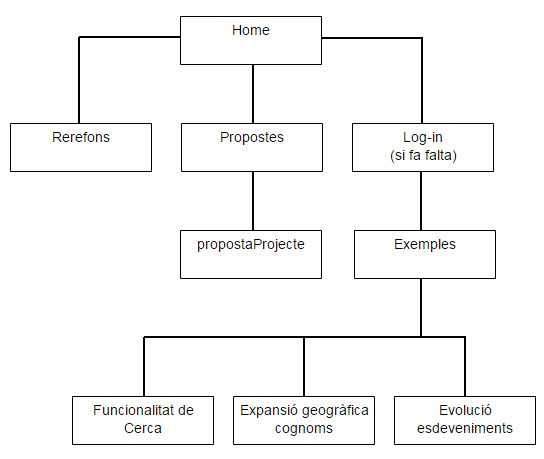
\includegraphics[scale=0.6]{10/01_estructuraWeb}
        \centering
        \caption{Diferents seccions de l'aplicació web}\label{fig:webStructure}
    \end{figure}

    Més endavant, s’explicarà més en detall en què consisteix cada una de les pàgines o seccions de la nostra aplicació web, però primer volem presentar l'estructura general o esquelet, que segueixen gairebé totes les pàgines del nostre web.

    La figura~\ref{fig:pageStructure} mostra l'esquema bàsic sobre el qual les pàgines són construïdes. Aquest pot ser descrit o desglossat en les següents seccions:

    \begin{enumerate}
        \item \textbf{Barra de navegació:} Permet desplaçar-se per les diferents seccions principals.
        \item \textbf{Capçalera de secció:} Conté el títol i subtítol de la pàgina sobre impressionat a una imatge relacionada.
        \item \textbf{Contingut principal:} El contingut principal i únic d'aquesta pàgina.
        \item \textbf{Footer:} Peu de pàgina. Inclou informació sobre el codi font del projecte, la llicència i la facultat d'informàtica de Barcelona.
    \end{enumerate}

    \begin{figure}[h]
        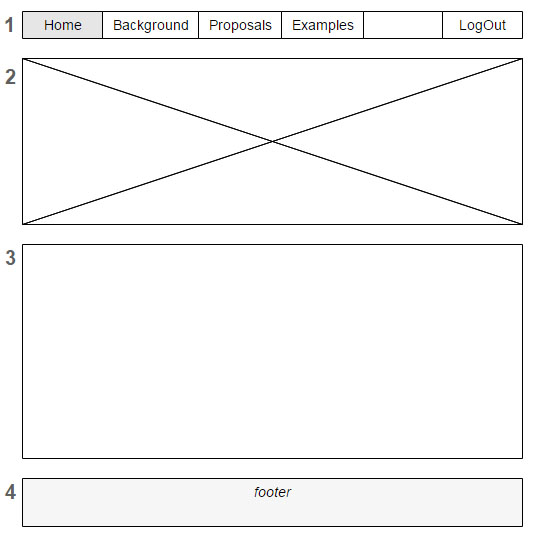
\includegraphics[scale=0.6]{10/02_pagesStructure}
        \centering
        \caption{Esquema bàsic de les pàgines implementades en el domini web}\label{fig:pageStructure}
    \end{figure}

    Convidem des de la memòria, als usuaris de l'aplicació web, a redimensionar la finestra web per tal d'observar com els continguts de cada pàgina s’adapten al dispositiu que els mostra.

    A continuació descriurem el contingut de cada secció o apartat que conforma la nostra aplicació web.

    \subsection{Home o pàgina principal}

    \paragraph{}
    La home és la primera pàgina que veu l'usuari quan entra a l'aplicació web. Aquesta no té cap altre propòsit que el de donar la benvinguda i enllaçar als diferents continguts.

    El bloc de contingut principal d’aquesta pàgina inclou enllaços i breus descripcions, a les tres seccions principals del projecte. A saber: rerefons, propostes de projecte i exemples d'implementació.

    La principal diferència entre la versió per dispositius mòbils i la d'escriptori és que la primera fa desaparèixer el subtítol, simplifica el títol, transforma la barra de navegació en una usable per dispositius mòbil i transforma la secció de contingut principal apilant-ne el contingut de cada una de les tres columnes que la conformen.

    \subsection{Rerefons}

    \paragraph{}
    La pàgina de rerefons conté la informació bàsica respecte a l'origen, context i motivacions, que ens van portar a realitzar aquest projecte. Consisteix en un breu resum, molt superficial, d’alguns dels apartats exposats en la primera secció de la memòria.

    El bloc de contingut principal d'aquesta pàgina consisteix en dos grans blocs de text. El primer, descriu el rerefons del projecte, mentre que el segon ofereix una petita descripció del context i motivacions.

    La principal diferència entre les versions d'escriptori i mòbil és que la segona presenta un títol més simple, la desaparició del subtítol i una barra de navegació adaptada a dispositius mòbils. L'estructura del contingut roman igual, això si, adaptat a la grandària del dispositiu que el conté. 

    \subsection{Propostes de projecte}

    \paragraph{}
    L'apartat de propostes de projecte recull les diferents propostes que han estat generades per servir com a projectes finals de carrera pels estudiants d'informàtica.

    El bloc de contingut principal per aquesta pàgina consisteix en dos blocs composts per petites caixes que contenen una imatge, un títol i una petita descripció de la proposta que representen. Cada una d'aquestes caixes enllaça també amb una pàgina que conté alguns detalls de la proposta.

    El primer bloc de caixes representa les propostes generades pels futurs estudiants, mentre que el segon bloc està format per les propostes relacionades amb els exemples implementats.

    Les principals diferencies entre les versions d'escriptori i dispositius mòbils, és que la segona presenta un títol simplificat, la desaparició del subtítol, la barra de navegació adaptada i diferent nombre de caixes per fila segons el dispositiu utilitzat. Tres columnes per escriptoris, dues per tauletes gràfiques i una per mòbils.

    \subsection{Detalls específics d'una proposta de projecte}

    \paragraph{}
    Com bé indica el nom de la secció, aquesta pàgina mostra els detalls específics de la proposta seleccionada des de la pàgina propostes.

    Les diferents propostes són totes generades des del mateix document HTML. És en aquest cas el servidor, l'encarregat d'enviar un conjunt d'informació diferent segons la proposta que ha estat seleccionada. Veurem en més detall com aquest procés funciona en futurs apartats d’aquesta secció.

    El bloc del contingut principal per cada una de les propostes, està conformat per una breu descripció del projecte i en alguns casos, certs exemples, preguntes o possibilitats d’extensió, que la proposta pot abordar. Les propostes també disposen d’una petita valoració numèrica, que representa una valoració de la dificultat d’execució de la proposta. Com més gran és el valor, més complexa.

    La versió d'escriptori i mòbil no es diferencien en grans aspectes excepte en l'adaptació del contingut a la pantalla del dispositiu i els típics canvis esmentats en els apartats anteriors sobre el títol, subtítol i barra de navegació.

    \subsection{Identificació amb FamilySearch}

    \paragraph{}
    Aquesta pàgina s'utilitza per assegurar que l'usuari no pot utilitzar els exemples sense identificar-se abans amb l’API de FamilySearch.

    La pàgina apareix quan l'usuari intenta accedir a la pàgina d'exemples o la pàgina d'un exemple en concret, però encara no s’ha identificat amb FamilySearch. La pàgina permet dues accions simples, tornar enredera (o a la home si s'ha accedit a la pàgina mitjançant la introducció directa de l'URL) o identificar-se amb FamilySearch.

    El procés d'identificació s'inicia mitjançant el llançament d'un pop-up, que obre la pàgina de FamilySearch. Aquesta demana la introducció del nom d'usuari i contrasenya. Un cop aquesta informació ha estat verificada, el servidor redirigeix a l'usuari a la pàgina que havia demanat accedir.

    La pàgina d'identificació tampoc pateix cap reestructuració especial del contingut quan es veu amb dispositius més petits. Simplement, s'adapta a la pantalla que la mostra i reorganitza els botons que permeten tornar endarrere o obrir el procés d’identificació.

    \subsection{Exemples implementats}

    \paragraph{}
    La pàgina d'exemples implementats permet a l'usuari descobrir les diferents eines que han estat implementades, per demostrar possibles interaccions amb l’API de FamilySearch i accedir a cada una d'elles.

    El bloc de contingut principal, segueix un estil molt similar a la pàgina propostes de projecte, descrita tres apartats endarrere. Aquesta, mostra per cada un dels exemples implementats un títol, una breu descripció i permet a l'usuari navegar cap a les pàgines que contenen les implementacions concretes.

    Les principals diferencies entre les versions d'escriptori i dispositius mòbils són exactament les mateixes que per la pàgina de propostes de projecte. És a dir, títol adaptat, eliminació del subtítol, adaptació de la barra de navegació i nombre de propostes per fila segons la grandària del dispositiu.

    Realment, aquestes dues pàgines tenen un comportament tècnic idèntic i l'únic que les diferencia és el concepte semàntic que representen i en conseqüència, el contingut.

    \subsection{Funcionalitats de cerca, expansió geogràfica d'un cognom i evolució d'esdeveniments}

    \paragraph{}
    Aquestes pàgines segueixen el mateix patró que la gran majoria de pàgines web de l’aplicació. Recordem que l'esquelet d’aquestes pàgines es mostrava en la figura\ref{fig:pageStructure} d'aquesta mateixa secció de la memòria.

    La gran diferencia, d'aquestes pàgines amb la resta és que la part del contingut principal és relativament més complexa i diferent per cada una d'elles. És per aquest motiu, que el comportament exacte de cada una d'aquestes pàgines serà exposat per separat a la secció onze de la memòria.

    Pel que fa a l'estructura en comú que comparteixen amb la resta de pàgines, les diferències entre la visualització entre dispositius mòbils i escriptori són les ja conegudes: minimització del títol, desaparició del subtítol i adaptació de la barra de navegació.


    \section{Fitxers de l'aplicació web i la seva funcionalitat}

    \paragraph{}
    En aquest apartat de la memòria volem presentar l'arbre d'arxius generats per tal de programar la pàgina web i exposar la funció que desenvolupa cada un d'ells en el marc de l'aplicació.

    Recordem que tot el codi programat per tal de fer funcionar l’aplicació web pot ser trobat a l'URL:

    \begin{displayquote}
        https://github.com/sinh15/pfc-family-search
    \end{displayquote}

    El conjunt de fitxers programats, representa un total de [línies codi] línies de codi, de les quals un XX\% són codi HTML, un XX\% codi Javascript i un X\% codi CSS.

    La taula~\ref{tab:codeFiles} mostra la localització relativa de cada arxiu i en descriu breument la seva funcionalitat.

    \begin{center}
             \csvreader[
                separator=comma,
                before table=\sffamily\small,
                longtable={p{4cm-2\tabcolsep}p{10cm-2\tabcolsep}},
                table head={\caption{Fitxers de codi de l'aplicació web}\label{tab:codeFiles}\\\toprule%
                    \headentry{m{4cm-2\tabcolsep}}{Arxiu}
                    & \headentry{m{10cm-2\tabcolsep}}{Funció}\\\midrule},
                late after line=\\\midrule,
                late after last line=\\\bottomrule,
             ]
             {./tables/10/codeFiles.csv}
             {name=\name,desc=\desc}
             {\name&\desc}
     \end{center}

    \section{Funcionament general de l'aplicació web}

    \paragraph{}
    L'objectiu d'aquest apartat és explicar com els diferents components de la web interactuen entre ells per tal de crear l'aplicació web desplegada al núvol.

    Com a suport a les explicacions que s'oferiran, la figura~\ref{img:appWorkflow} mostra un diagrama amb els components principals de l'aplicació, com interactuen entre ells i els principals formats de dades que intercanvien.

    \begin{figure}
        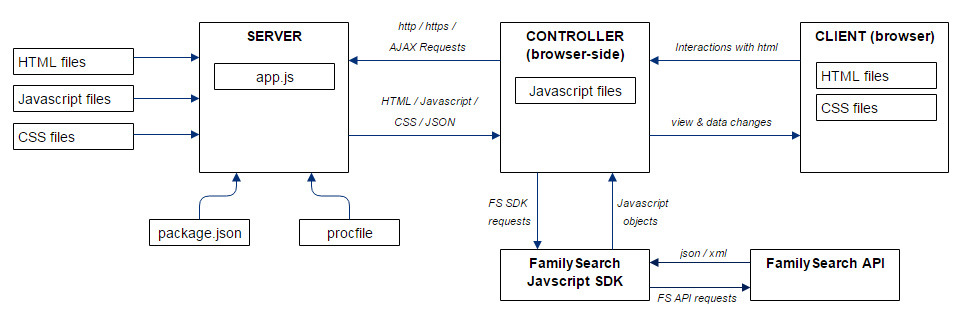
\includegraphics[scale=0.6, angle=90]{10/03_applicationWorkingFlow}
        \centering
        \caption{Comunicació entre els diferents components de l'aplicació web}\label{img:appWorkflow}
    \end{figure}

    En la imatge es poden observar les capes Servidor, Controlador i Client, que conformen l'arquitectura en tres capes explicada en seccions anteriors. També es pot observar el Javascript SDK, del que es detalla com es comunica amb l'API de FamilySearch i a quina capa de l'aplicació es troba connectat.


    \subsection{Creació del servidor}

    \paragraph{}
    L'aplicació comença a funcionar quan aquesta és executada en els servidors al núvol de Heroku, la plataforma d'hostalatge. La configuració del servidor es realitza mitjançant els fitxers \emph{Procfile} i \emph{package.json}, que s'encarreguen d'assegurar que tots els complements Javascript necessaris siguin instal·lats i s'executi el fitxer \emph{app.js} per arrancar i configurar el servidor.

    Quan la configuració del servidor acaba, aquest es troba preparat per començar a rebre peticions dels usuaris.


    \subsection{Accés a una pàgina del domini web}

    \paragraph{}
    Quan un usuari demana carregar la pàgina inicial de la nostra aplicació, una petició HTTP o HTTPS és generada i enviada cap al servidor a través del navegador del client.

    Quan el servidor la rep, l'avalua i en cas d'èxit, retorna al client els fitxers processats necessaris perquè el navegador pugui mostrar la pàgina demanada i carregar totes les funcionalitats o interaccions possibles d'aquesta al controlador.


    \subsection{Interacció amb l'API de FamilySearch}

    \paragraph{}
    El moment en què l'usuari vol interactuar amb l'API de FamilySearch, aquest es veu forçat a interactuar primer amb un element del codi HTML per comunicar l’acció a realitzar. Per exemple, el botó de cerca de la funcionalitat d'evolució temporal d'esdeveniments.

    Quan el controlador detecta que el botó de cerca ha estat pressionat, captura l'esdeveniment i avalua la petició. En cas que no es detecti cap problema ni error en els paràmetres introduïts, el controlador realitza una crida asíncrona al SDK de FamilySearch i n'espera la resposta.

    De forma transparent a l'aplicació web, el SDK es comunica amb l’API de FamilySearch i si no hi ha cap problema en la comunicació i la petició és vàlida, aquesta retorna les dades demanades en format XML o JSON. Posteriorment, el SDK transforma la resposta de l’API en un objecte Javascript amb funcions de conveniència que facilitaran l'accés a les dades de la resposta i el retorna al controlador.

    En el moment que el SDK retorna l'objecte, la promesa pendent de resolució que havia creat el controlador és resolta i l'objecte retornat pel SDK passa a ser accessible. Arribats a aquest punt, el controlador processa i transforma les dades contingudes a l'objecte de la forma desitjada i un cop finalitzades les operacions necessàries, modifica la vista del client introduint els canvis pertinents en aquesta.


    \subsection{Interacció amb elements del HTML}

    \paragraph{}
    Quan els usuaris interactuen amb elements bàsics del HTML, per exemple, quan interactuen amb les caixes que permeten expandir o plegar seccions del formulari en les funcionalitats de cerca o evolució geogràfica de cognoms, la resposta a realitzar per part del controlador és bastant simple.

    En el moment que el controlador detecta que s'ha interactuat amb algun dels elements que escolta, captura l'esdeveniment, avalua com s'ha de procedir segons el context de l'acció, en el cas de l’exemple, plegar o desplegar contingut d'un formulari i realitza de forma immediata els canvis a la vista del navegador.


    \subsection{Conclusió}

    \paragraph{}
    Els casos d'ús que s'han cobert en els apartats anteriors són relativament simples, però són una mostra representativa del conjunt d'accions diferents a les quals l'aplicació pot haver de fer front.

    Esperem que aquesta secció hagi servit per il·lustrar el funcionament general de la web i com els diferents components interactuen entre ells. La resta d’accions possibles en el web, requerint més o menys complexitat per part del controlador, segueixen una de les tres rutes descrites en els apartats anteriors, per tal de ser satisfetes.


    \section{Procés de certificació}

    \paragraph{}
    Per tal de poder connectar les aplicacions desenvolupades per tercers al conjunt de dades oficial de FamilySearch, aquestes aplicacions han de ser sotmeses a un procés de certificació.

    Les aplicacions poden ser certificades per l'ús comercial o per ús limitat. Les Apps que volen ser certificades només per ús limitat, requereixen un anàlisis tècnic sobre el seu funcionament, mentre que de les aplicacions d'ús comercial també són analitzades des d'un punt de vista de negoci i marketing. Com a contrapartida, les aplicacions d'ús limitat no poden aparèixer a la galeria d'aplicacions.

    Hi ha tres tipus de certificacions principals:

    \begin{itemize}
        \item \textbf{Certificació de lectura:} L'aplicació ha de ser certificada per la lectura de tots aquells recursos als quals accedeix. També cal que compleixi amb certs estàndards del procés d'identificació.
        \item \textbf{Certificació d'escriptura:} En cas que l'aplicació realitzi operacions d'escriptura, aquestes també hauran de ser revisades per part de FamilySearch.
        \item \textbf{Certificació per transferència d'arxius en grans quantitats:} Per aquelles organitzacions que tinguin permís per accedir als protocols de transferència de dades en grans quantitats, cal certificar i revisar, conjuntament amb FamilySearch, les operacions realitzades contra aqueta API.
    \end{itemize}

    \paragraph{}
    Es veuran més detalls sobre el procés de certificació en la part pràctica de la memòria del projecte.

    Un cop una aplicació ha estat certificada, en cas que aquesta modifiqui les operacions de lectura o escriptura que realitza, caldrà tornar a certificar-la abans de desplegar els canvis a producció.

    Existeix un procés encarregat de controlar que es compleixen els estàndards marcats per FamilySearch i en cas de no complir-los, pot significant el retirament dels drets d'accés a producció.

    Per acabar aquesta secció, comentar que mantenir una relació formar amb FamilySearch, proporciona certs beneficis com aparèixer en les seves galeries d'aplicacions i poder utilitzar el logotip d'aplicació certificada, entre altres petits avantatges.

    \section{Google Analytics}

    \paragraph{}
    Google Analytics és un servei d'analítica web, proporcionat per Google, que s'encarrega de monitorar i reportar dades relatives al tràfic d'una aplicació web o aplicació mòbil.

    Mitjançant una implementació relativament simple, és possible emmagatzemar informació relativa a les pàgines visitades, la navegació entre pàgines, els sistemes operatius utilitzats, informació sobre els diferents navegadors, resolucions de pantalla, dispositius mòbils utilitzats i interaccions bàsiques dels usuaris amb les diferents pàgines del web.

    Gran part d'aquesta informació és capturada de forma automàtica, per Google Analytics, pel simple fet d'incloure el `snippet' de codi de l'eina a les nostres pàgines del domini web. A canvi, es disposa de moltes variables que poden ser creuades per tal d'analitzar el rendiment del domini web i l'ús que li donen els usuaris.

    De totes maneres, no s'espera que la nostra aplicació web disposi de grans quantitats de tràfic i la implementació de Google Analytics no ha vingut donada pel fet de poder analitzar el rendiment tècnic o d'usabilitat de l'aplicació, sinó per poder controlar el funcionament de la integració amb l'API de FamilySearch.

    Durant el desenvolupament de l'aplicació, mentre interactuàvem amb l'entorn sandbox de l'API, ens vàrem adonar que durant diversos dies i inclòs a vegades, períodes de tres o quatre dies, l'entorn no funcionava i les peticions llençades contra l'API eren cancel·lades.

    Per tal de poder monitorar en tot moment el funcionament de les interaccions dels usuaris amb l'API, s'ha utilitzat la funcionalitat de Google Analytics que permet enviar esdeveniments personalitzats, que o bé reflecteixen accions dels usuaris o condicions que s'han donat en l'aplicació web o mòbil.

    En concret, s'han creat quatre nivells d'esdeveniments diferents per cada una de les funcionalitats principals que interactuen amb l'API de FamilySearch:

    \begin{itemize}
        \item \emph{Formulari incorrecte:} En el cas que un usuari intenti llençar una petició contra l'API i aquesta no s'iniciï perquè el formulari contenia errors, es marca l'intent amb una etiqueta de formular incorrecte.
        \item \emph{Petició llençada:} Si la validació de tots els camps és correcta, s'envia un esdeveniment indicant que un intent de connexió amb l'API, s'ha llençat amb el SDK de FamilySearch i els paràmetres d'aquesta petició.
        \item \emph{Petició rebutjada:} En cas que el SDK no pugui resoldre la petició per qualsevol motiu, s'enregistra un esdeveniment que indica el rebuig de la petició i n'especifica el motiu (Per exemple, timeout, no existeix el recurs, excés de peticions en un període limitat de temps, etcètera).
        \item \emph{Petició retornada amb èxit:} Quan el SDK processa la petició i retorna resultats, s'envia un esdeveniment d'èxit.
    \end{itemize}

    Mitjançant l'existència d'aquests quatre nivells per cada una de les funcionalitats implementades, podrem conèixer l'estat de la connexió amb l'API de cada una d'elles, amb un esforç relativament baix.

    La figura~\ref{img:factsEvents} mostra els diferents quatre nivells d'esdeveniments per la funcionalitat evolució d'esdeveniments. Com es pot veure en la imatge, Google Analytics captura quantes vegades s'ha donat un esdeveniment concret en el període de temps definit i quantes sessions l'han contingut en algun moment donat.

    \begin{figure}
        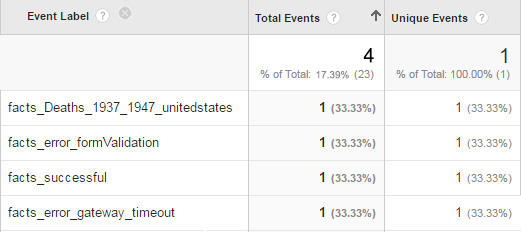
\includegraphics[scale=0.6]{10/04_factsEvents}
        \centering
        \caption{Exemple d'esdeveniments de la funcionalitat evolució d'esdeveniments}\label{img:factsEvents}
    \end{figure}

    A continuació, també citem els diferents exemples mostrats en la figura [] i hi afegim algun comentari.

    \begin{itemize}
        \item \textbf{Formulari incorrecte:} \emph{facts\_error\_formValidation}. Esdeveniment que s'envia quan la petició no s'ha arribat a processar perquè la configuració dels paràmetres no era correcta.
        \item \textbf{Petició llençada:} \emph{facts\_Deaths\_1937\_1947\_unitedstates}. Com es pot veure, quan es llança una petició contra l'API, també capturem el tipus d'esdeveniment cercat (defuncions), les dates per les quals s'ha cercat (1937-1947) i el país seleccionat (Estats Units).
        \item \textbf{Petició rebutjada:} \emph{facts\_error\_gateway\_timeout}. Aquest és un exemple dels esdeveniments que poden ser retornats quan l'API no ha pogut processar la petició.
        \item \textbf{Petició retornada amb èxit:} \emph{facts\_successful}. Esdeveniment que s'envia quan tot ha funcionat com s'esperava i l'API ha retornat resultats.
    \end{itemize}

    Els exemples d'esdeveniments anteriors, serveixen per demostrar el potencial que pot arribar a desencadenar una eina d'analítica web com Google Analytics.

    A part dels esdeveniments relatius a les funcionalitats implementades, que interactuen amb l'API de FamilySearch, també s'han implementat esdeveniments per controlar els intents d'identificació contra FamilySearch satisfactoris, les peticions de desconnexió, posicions dels exemples i propostes de projecte amb les que s'ha interactuat, interaccions amb la barra de navegació, posició de la persona seleccionada en la llista de resultats de la funcionalitat de cerca, etcètera.

    Tot i que el conjunt d'informació que s'ha exposat fins ara relativa a Google Analytics podria ser considerada simple, no creiem que sigui l'objectiu de la memòria entrar en molt més detall en les possibilitats d'una eina d'analítica web com aquesta, doncs realitzar una proposta profunda i exhaustiva de les possibilitats de monitoratge d'una web com la implementada, bé podria ser un projecte propi.

    \section{Optimitizació d'imatges}

    \paragraph{}
    Un dels elements més importants quan es desenvolupa una pàgina web és que aquesta carregui de forma ràpida. La diferència entre una pàgina lenta i una de ràpida, s'acaba traduint generalment en una pàgina web sense usuaris o amb usuaris.

    No era un objectiu del projecte fer una pàgina web el més optimitzada possible, ja que els coneixements tècnics necessaris requereixen temps per ser adquirits. No obstant això, sí que es volia realitzar les optimitzacions més típiques, que també solen ser les que endarrereixen més la càrrega de les pàgines web.

    Aquest apartat, cobra relativa importància, si tenim present que estem utilitzant un servei d'hostalatge gratuït i que per tant, la velocitat de resposta del servidor, no és de les millors del mercat.

    La manca d'optimització en les imatges sol ser un dels factors que més afecta a l'hora de carregar una pàgina web. Els programes de disseny utilitzats per generar imatges de gran qualitat, solen emmagatzemar més informació que la perceptible per l'ull humà, en circumstàncies normals.

    És per aquest motiu que optimitzar les imatges, els arxius més grans a descarregar de forma general en una web, esdevé un procés relativament comú.

    Per optimitzar les imatges de la nostra aplicació web s'ha utilitzat l'aplicació Optimizilla. Aquesta eina, penjada al núvol, utilitza una combinació de tècniques d'optimització i compressió amb pèrdues, per tal de reduir al màxim el pes d'imatges JPG i PNG, sense reduir el nivell de qualitat perceptible per l'ull humà.

    La utilització d'aquesta eina ha reduït, de forma aproximada, el 60-80\% del pes de totes les imatges que s'utilitzen en l'aplicació web. Fet considerable, si tenim en compte que no s'ha reduït la qualitat perceptible d'aquestes.

    \section{Hosting de l'aplicació}

    \paragraph{}
    Com ja s'ha indicat en el primer apartat d'aquesta secció de la memòria, l'aplicació es troba accessible a través del domini:

    \begin{displayquote}
        https://pfc-family-search.herokuapp.com/
    \end{displayquote}

    Hem escollit la plataforma Heroku per desplegar l'aplicació, ja que oferia un ampli ventall d'eines i documentació, que resultaven ideals per un desenvolupador novici de la plataforma Node.js.

    No obstant això, no van ser només aquestes facilitats i eines les que ens van portar a desplegar l'aplicació a Heroku, sinó també el fet que el seu pla de hosting gratuït s'ajustava en gran mesura al que el projecte requeria i en cas d'acabar necessitant més, sempre existia la possibilitat d'augmentar la capacitat de processat necessària.

    Les característiques que més ens van atreure de la plataforma Heroku es presenten d'una en una en els següents apartats.

    \subsection{Fàcil configuració}

    \paragraph{}
    Per una aplicació simple com la desenvolupada per aquest projecte, no fa falta canviar res en el codi de la nostra aplicació per tal de desplegar-la a Heroku. Només hem d'incloure un nou fitxer, a la carpeta arrel del projecte i amb el nom \emph{Procfile}, que indica el tipus d'aplicació i la comanda que ha ser utilitzada per tal d'iniciar-la.

    En el nostre cas, el fitxer \emph{Procfile} conte la següent línea de codi:

    \begin{displayquote}
        > web: node app.js
    \end{displayquote}


    \subsection{Fàcil desplegament al núvol}

    \paragraph{}
    La plataforma Heroku es troba molt ben integrada amb Github, l'eina que hem utilitzat per mantenir sincronitzats els desenvolupaments en les diferents estacions de treball. Gràcies a aquesta integració, Heroku disposa d'una comanda que ens permet afegir un remot, a la carpeta del nostre projecte.

    \begin{displayquote}
        > heroku git:remote -a pfc-family-search
    \end{displayquote}

    Un cop tenim el remot de Heroku configurat, de la mateixa forma que podem enviar el codi de la nostra estació de treball al núvol, el podem enviar a Heroku per tal de desplegar la nostra aplicació web. Això és tan fàcil com llençar la següent instrucció.

    \begin{displayquote}
        > git push heroku master
    \end{displayquote}


    \subsection{Entorn de proves local}

    \paragraph{}
    A part de l'entorn de proves local que podem configurar mitjançant la instal·lació de Node.js en el nostre sistema, Heroku també ens permet simular un entorn de producció Heroku, en l'àmbit local. S'aconsegueix mitjançant la següent instrucció:

    \begin{displayquote}
        > heroku local web
    \end{displayquote}

    Tot i que no aporta gaires diferències respecte a desplegar l'aplicació en local mitjançant Node.js de la forma convencional, pot esdevenir útil sota certes circumstàncies.


    \subsection{Decent versió gratuita}

    \paragraph{}
    Durant tot el procés de desenvolupament, l'aplicació es trobava sota el paquet de funcionalitats gratuït ofert per Heroku.

    Aquest ofereix les següents funcionalitats:

    \begin{itemize}
        \item Desplegament des de repositoris GIT.
        \item Actualitzacions automàtiques.
        \item Auto reparació d'aplicacions.
        \item Logs del sistema.
        \item Nombre de processos diferents suportats: 2
        \item 1000 hores mensuals de \emph{dyno} actius. L'aplicació s'adorm després de 30 minuts d'inactivitat.
        \item Dominis personalitzables.
        \item 512MB de RAM
    \end{itemize}


    \subsection{Fàcil escalatge de l'aplicació}

    \paragraph{}
    En cas que es desitgi millorar la capacitat de concurrència de l'aplicació, per poder rebre i processar més peticions en paral·lel i realitzar més processos diferents al mateix temps, aquesta és fàcilment escalable mitjançant la inclusió de nous \emph{dynos}.

    Els \emph{dynos} són els contenidors que executen les comandes dels usuaris. Per la nostra aplicació web, bàsicament es necessiten \emph{dynos} que processin el tràfic HTTP i HTTPS. Gràcies al fet que el nostre servidor és bastant simple (hem posat la lògica d'interacció amb l'API de FamilySearch a la capa del controlador) és probable que no faci falta augmentar el nombre de \emph{dynos} inicial.

    De totes maneres, aquest és fàcilment escalable mitjançant una simple comanda, sempre i quan el nostre pla contractat amb Heroku no sigui el gratuït. Si volem augmentar, per exemple, a 2 el nombre de \emph{dynos} disponibles, executaríem la següent comanda:

    \begin{displayquote}
        > heroku ps:scale web=2
    \end{displayquote}

